
\documentclass[PICOReport.tex]{subfiles}

\begin{document}

%Enumerate the various signals in polarization. Use the frequency band + signals figure. The challenge is to dig out the faintest of all signals, the one due to $r$. This sets the tone for the entire 'signal decomposition' or 'component separation'.  Removing the galactic signal to unmask $r \lesssim 0.001$ is a challenge for all future experiments searching for $r$ at that level, and is a strong advantage of a space platform. The physics of galactic signals suggests complexities in their combined emission properties; the level of this complexity is not known. } 

%\comblue{Let's make clear that there are numerous signals that need to be separated; rather than a 'signal' and 'foregrounds'.} 
Diffuse Milky way emissions dominate the sky's polarized intensity on the largest angular scales; see Figure~\ref{fig:pico-channels-and-fg}. \comor{also reference to Figure 1?} Even in the cleanest, smaller patches of the sky, far from the galactic plane and thus relatively low in galactic emissions, their levels are expected to dominate the CMB inflationary $BB$ signal for $r \lesssim 0.01$, and overwhelm it for $r \lesssim0.001$; see Figure~\ref{fig:pico-channels-and-fg}. Foreground separation together with control of systematic uncertainties is the challenge facing any next decade experiment attempting to reach these levels of constraints on $r$.

The challenge would be easily surmountable if Galactic emissions were already precisely characterized, or were  known to have simple, fittable emission laws. But neither is true. Until recently, the spectrum of Galactic synchrotron emission, arising from free electrons spiraling around Galactic magnetic fields, was modeled as a power law $I_{\rm sync} \propto \nu^{\alpha},$ with $\alpha \simeq -1$ (in brightness units). The spectrum of Galactic dust emission, arising from emission by Galactic dust grains, was modeled as $I_{\rm dust} \propto \nu^{\beta} B_\nu(T_{\rm dust}),$ where $\beta \simeq 1.6$, $T_{\rm dust} \simeq 19$\,K, and $B_\nu(T)$ is the Planck function. \comor{the values are averages across the sky?} However, WMAP and Planck observations have shown that neither emission law is universal; that spectral parameters vary with the region of emission \comor{is that true? is there evidence from Planck; add references}. Also, while both emission laws are well-motivated phenomenological descriptions, the fundamental physics of emissions from grains of different material, sizes and temperatures, and of electrons spiraling around magnetic fields implies that they are not expected to be exact, nor universal. 

We know that we don't know enough about synchrotron and dust emission. We know even less about the polarization level of 'anomalous dust emission', an excess of dust emission at frequencies between 10 and 100~GHz, and of infra-red sources. Depending on reasonable levels of polarization assumed their contributions to the total polarized signal may be appreciable or negligible (for $r\lesssim 0.001$)~\citep{??}.  

%At the level of accuracy required by the anticipated stringent constraints on $r$, one must learn from the data themselves. 
%, and refine the models and the component separation techniques to reach a level of residual foreground contamination of 0.01\ % 

 

%

%%%%%%%%%%%%%%%%%%%%%%%%%%%%%%%%%%%
\subsubsection{The PICO component separation challenge}
%%%%%%%%%%%%%%%%%%%%%%%%%%%%%%%%%%%

The baseline design of PICO has 21 channels observing the sky in the 20\,GHz to 800\,GHz frequency range (Fig.~\ref{fig:pico-channels-and-fg}). By analysing how the total emission varies across frequency bands, one can infer the detailed emission properties of the various emission components, form linear combinations of the observations that maximise the contribution of a component of interest while minimising contamination by the others and by instrumental noise, and understand the properties of the foregrounds to evaluate potential residuals in the CMB B-mode map. Various such techniques have been successfully used in previous CMB observations such as those of the Planck mission. Building on this existing expertise, we have carried out map based simulations within a ``data challenge'' framework to assess the capacity of PICO to measure the main signal of interest (CMB primordial B-modes). In this process one group prepares sets of simulated maps for different models of foreground emission of varying complexity from optimistic to pessimistic, which are placed in a shared area. These are then re-analyzed by multiple individuals and groups employing various different component separation algorithms.

\begin{figure}
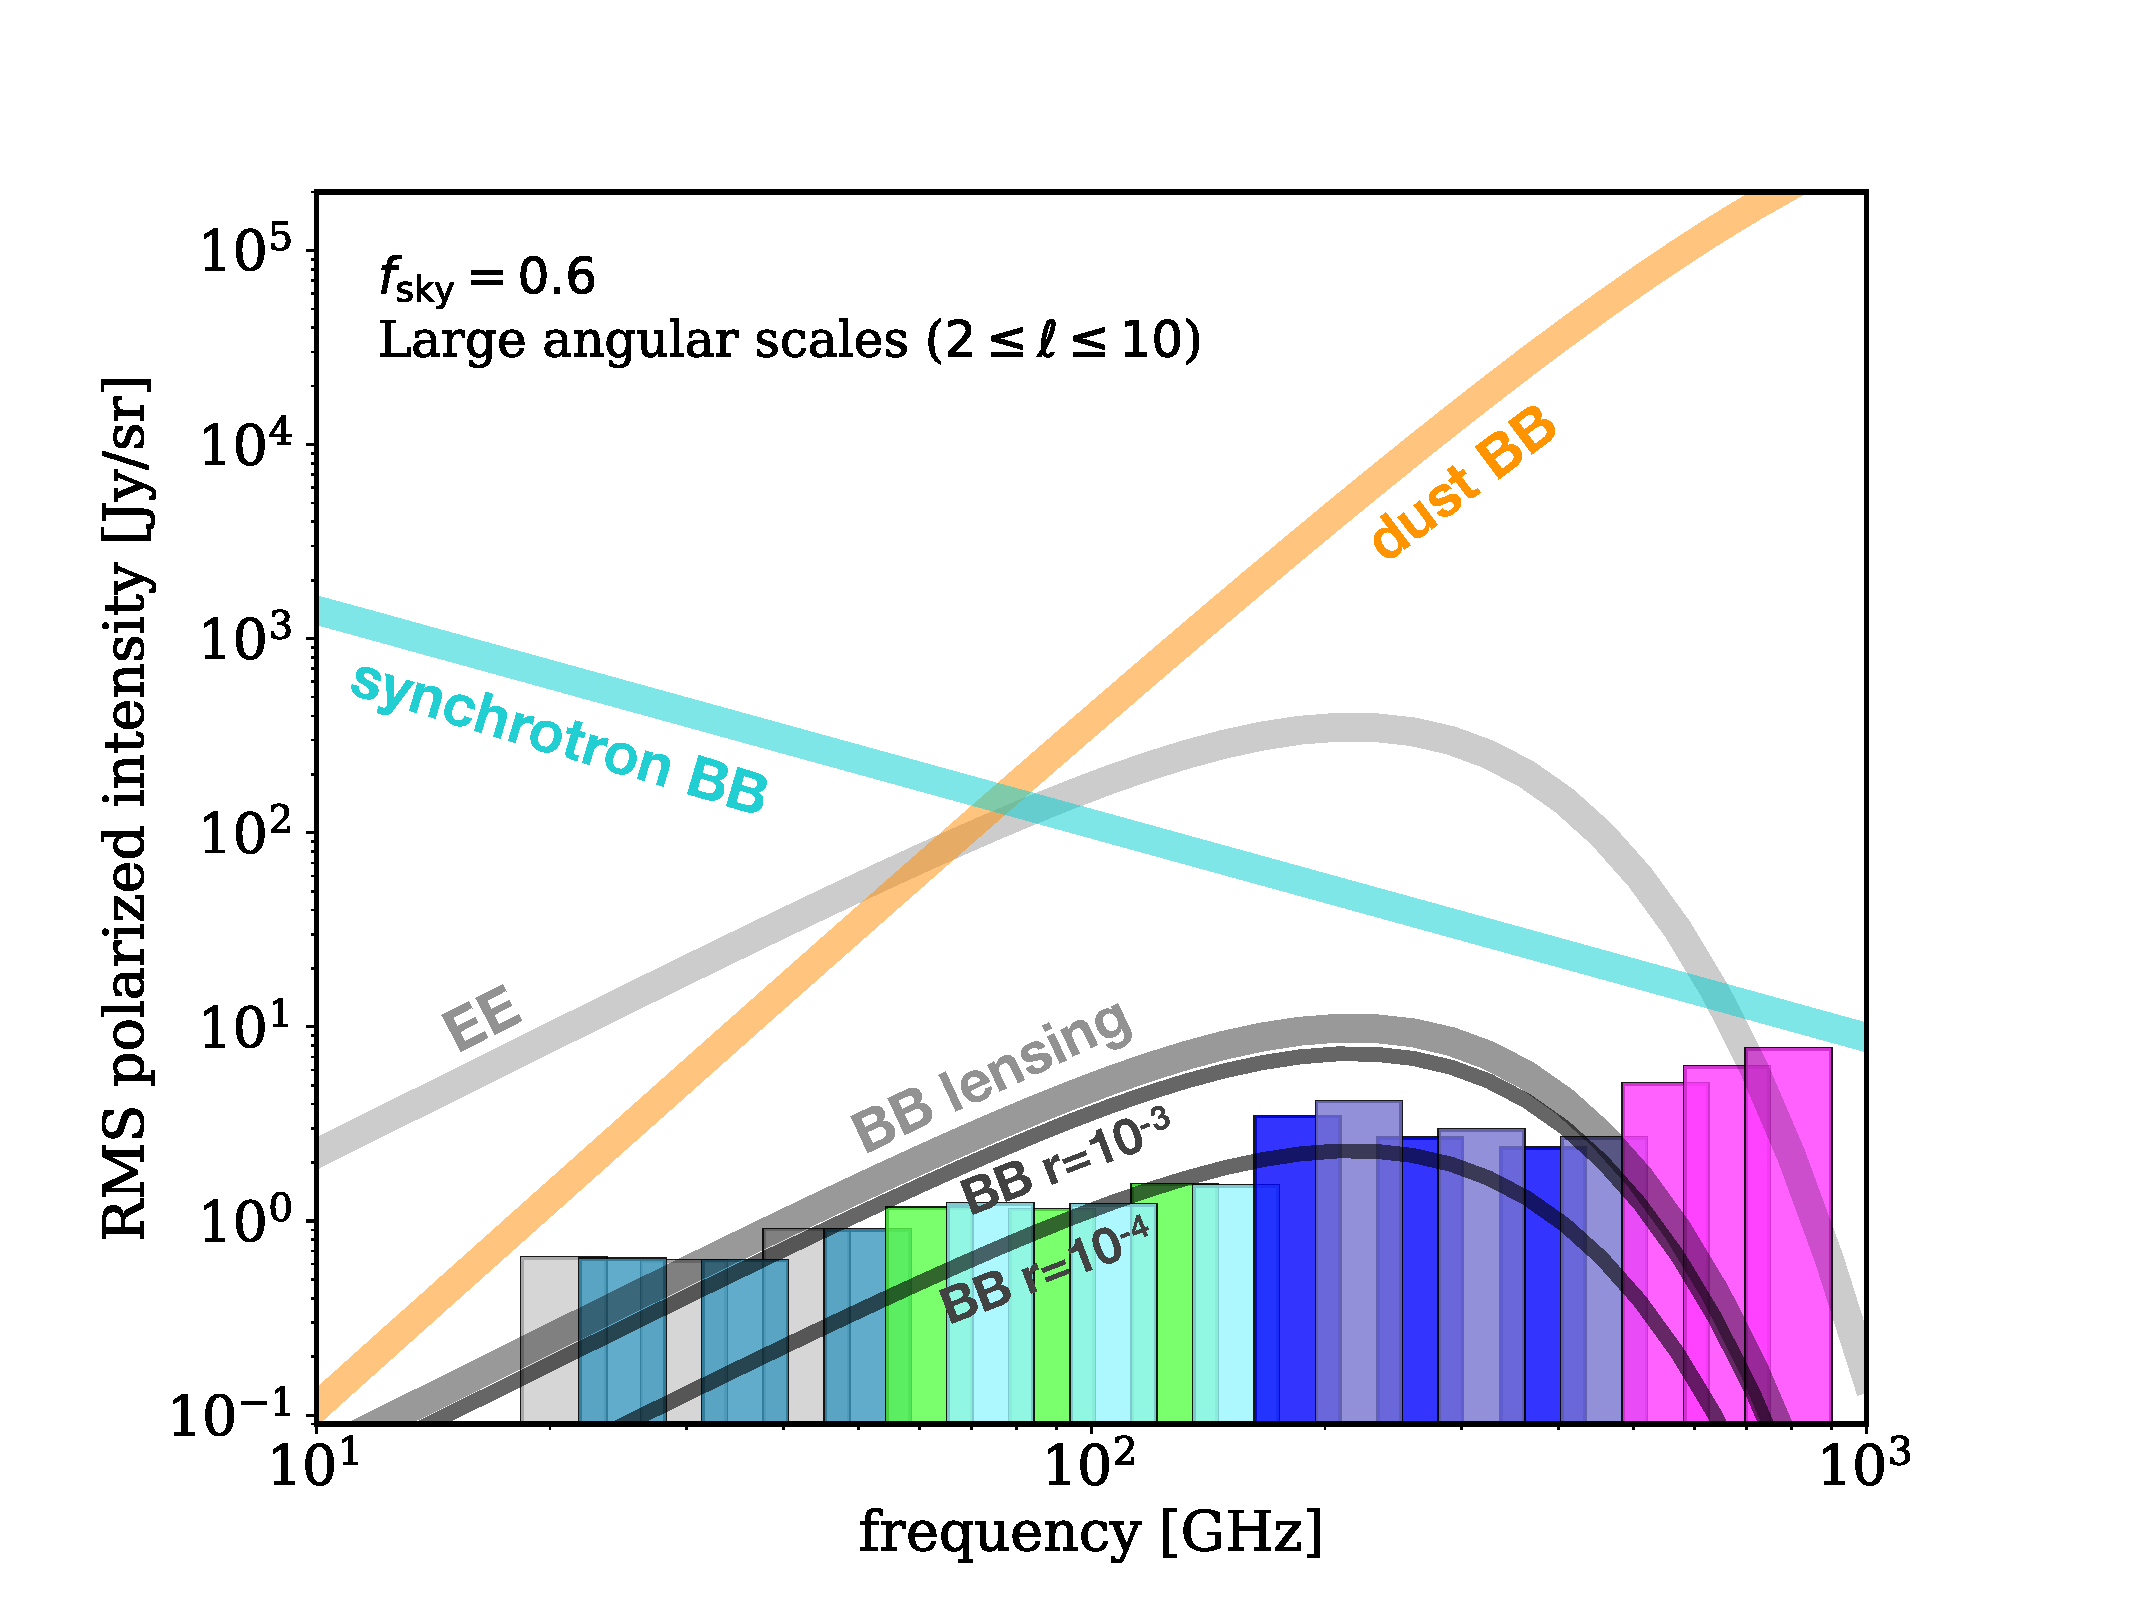
\includegraphics[width=0.49\textwidth,angle=0]{images/sensitivity_vs_frequency_Jun29th_2018_large.pdf}
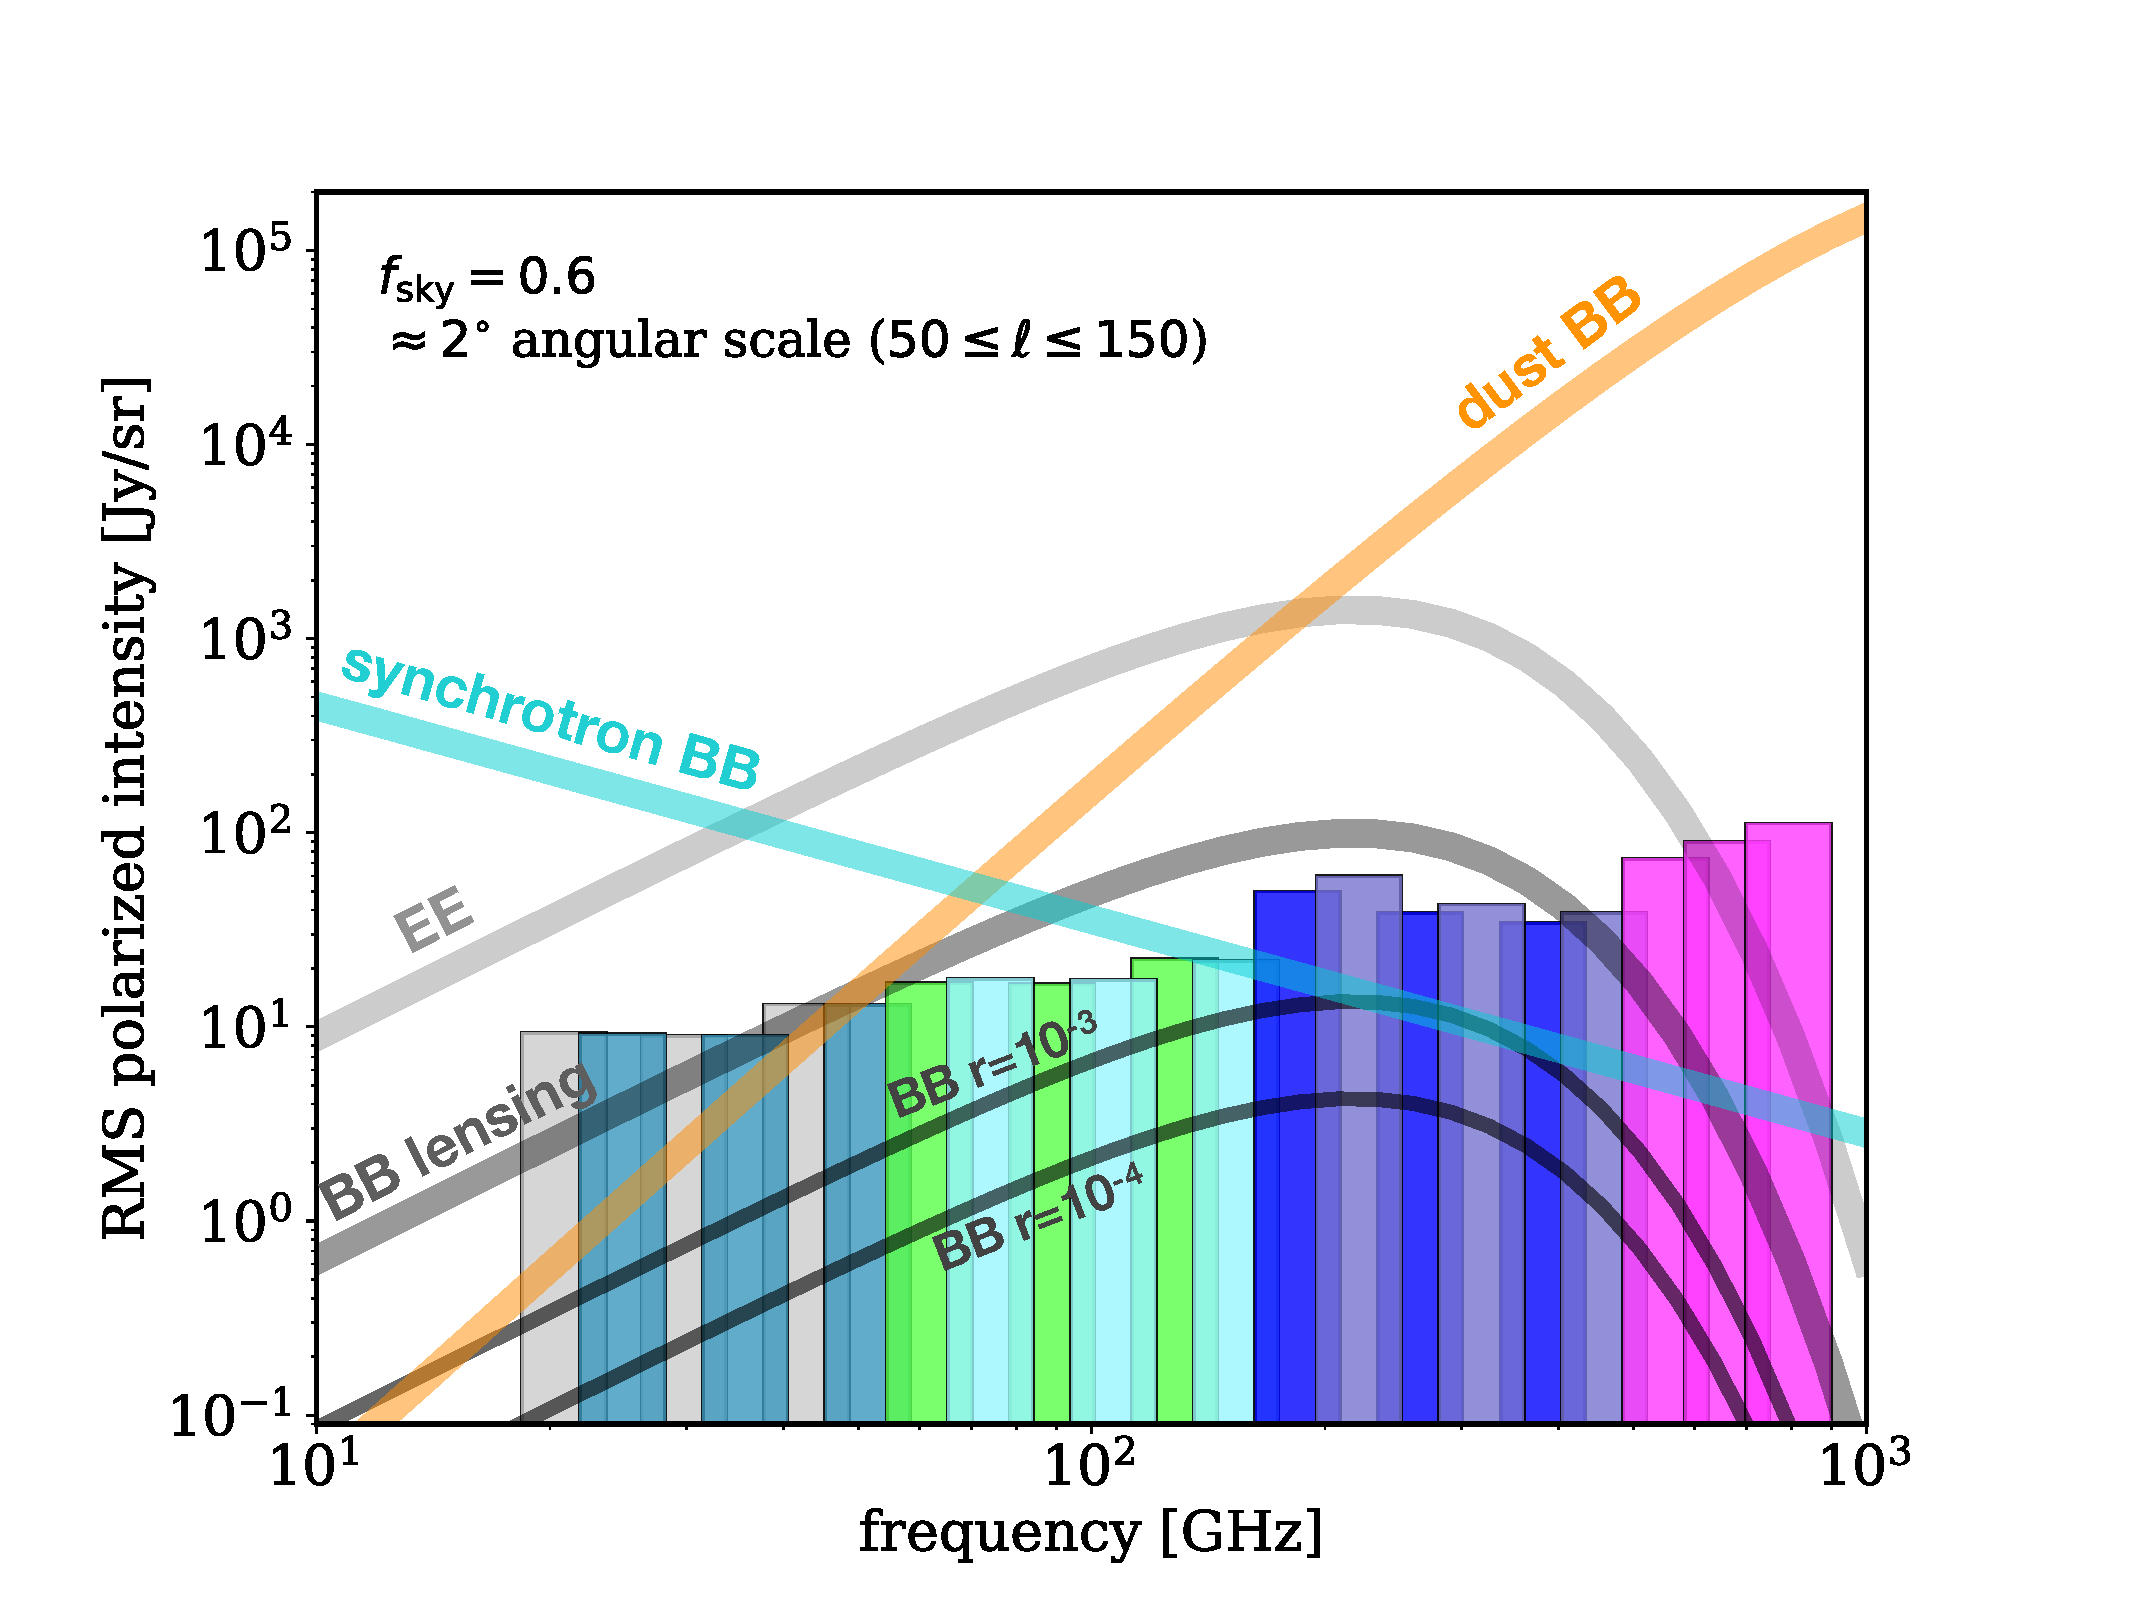
\includegraphics[width=0.49\textwidth,angle=0]{images/sensitivity_vs_frequency_Jun29th_2018_2deg.pdf}
\caption{Polarization B modes of Galactic synchrotron and dust, compared to CMB polarization E-modes and B-modes of different origin, for two values of the tensor-to-scalar ration $r$. The location and sensitivity of the PICO frequency channels is shown as vertical bands. Left: integrated r.m.s. emission on the largest angular scales ($2\leq \ell \leq 10$), corresponding to the reionization peak; Right, integrated r.m.s. emission on $\simeq 2^\circ$ angular scales ($50 \leq \ell \leq 150$), corresponding to the expected recombination peak in CMB primordial B modes.}
\label{fig:pico-channels-and-fg}
\end{figure}

%%%%%%%%%%%%%%%%%%%%%%%%%%%%%%%%%%%
%\subsubsection{The PICO simulated observations}
%%%%%%%%%%%%%%%%%%%%%%%%%%%%%%%%%%%

Several different models of foreground emission have been used for the PICO data challenge, from simple Gaussian realizations of synchrotron and dust at the level observed in the BICEP2 field, scaling rigidly in frequency with a single modified blackbody, to models in which the spectral parameters of foregrounds can vary across the sky and along the line of sight, AME can be 2\% polarized, dust polarization can rotate slightly as a function of frequency by reason of projection effects, or the dust SED can depart from a simple modified blackbody. All foreground maps are generated at native HEALPix resolution {\tt nside=512}. They are generated using PySM and/or PSM codes.
%
The CMB is generated as realizations of lensed-$\lambda$CDM from the Planck simulations data set, with primordial B-modes at the $r=0.003$ level. PICO noise is simulated as Gaussian uniform on the sky and uncorrelated from pixel to pixel, at the appropriate levels for each of the 21 PICO bands. 

%%%%%%%%%%%%%%%%%%%%%%%%%%%%%%%%%%%
%\subsubsection{Component separation methods}
%%%%%%%%%%%%%%%%%%%%%%%%%%%%%%%%%%%

Observations from the challenge are analyzed with a variety of well-established component separation methods that rely on various approaches to model the data and to separate the various emissions. These methods can be classified in two broad categories: correlation methods, which exploit the fact that foreground emission is strongly correlated from frequency to frequency, but uncorrelated with the CMB, and parametric methods, which model the sky emission using specific (parametric) emission laws, and use spectral fits in independent pixels or sky regions to infer the amplitude and spectral parameters of each of the components in the sky. Correlation methods include the SEVEM algorithm, and variants of the Internal Linear Combination (ILC) algorithm, such as the needlet space ILC (NILC) and a version generalised to multidmensional components (GNILC). Parametric methods include the Commander algorithm and the X-forecast method.

%%%%%%%%%%%%%%%%%%%%%%%%%%%%%%%%%%%
\subsubsection{Results}
%%%%%%%%%%%%%%%%%%%%%%%%%%%%%%%%%%%

%%%%%%%%%%%%%%%%%%%%%%%%%%%%%%%%%%%
\subsubsection{Discussion}
%%%%%%%%%%%%%%%%%%%%%%%%%%%%%%%%%%%


\end{document}

%\begin{figure}[!htb]
%\centering
%
\includegraphics[width=4cm]{images/example}
%\caption{example}
%\label{fig:im_3}
%\end{figure}
